\documentclass[convert={density=300,size=1080x800,outext=.png}]{standalone}
\usepackage{tkz-graph}
\usetikzlibrary{arrows,positioning,shapes,shapes.multipart,patterns,mindmap,shadows}
\usepackage{xcolor}
\usepackage{helvet}
\renewcommand{\familydefault}{\sfdefault}


\begin{document}

\footnotesize
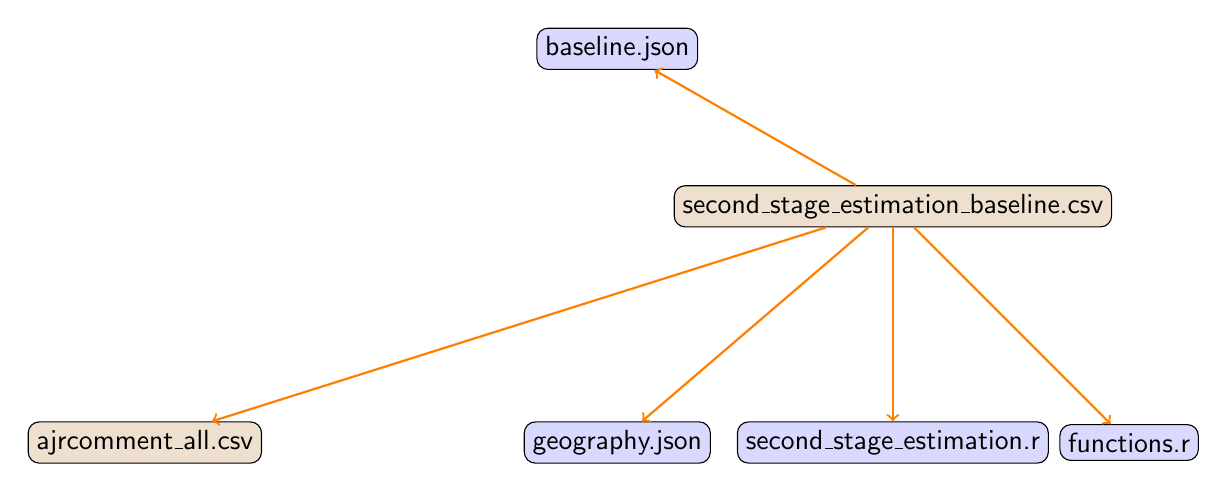
\begin{tikzpicture}[every node/.style={
    rectangle,
    rounded corners,
    inner sep=3pt,
    draw,
    fill=brown!25
}]
	    \node (ajrcomment_all_csv) [shift={(-2, 0)}]
	{
		ajrcomment\_all.csv
	};

	%analysis

	\node (geography_r) [fill=blue!15, shift={(4, 0)}]
	{
		geography.json
	};
	\node (baseline_r) [fill=blue!15, shift={(4, 5)}]
	{
		baseline.json
	};
    \node (functions_r) [fill=blue!15, shift={(10.5, 0)}]
    {
        functions.r
    };

    \node (second_stage_estimation_baseline_csv) [shift={(7.5, 3)}]
    {
        second\_stage\_estimation\_baseline.csv
    };


    \node (second_stage_estimation_r) [fill=blue!15, shift={(7.5, 0)}]
    {
        second\_stage\_estimation.r
    };




    \draw[->, orange, thick] (second_stage_estimation_baseline_csv) to (second_stage_estimation_r);
    \draw[->, orange, thick] (second_stage_estimation_baseline_csv) to (geography_r);
    \draw[->, orange, thick] (second_stage_estimation_baseline_csv) to (ajrcomment_all_csv);
    \draw[->, orange, thick] (second_stage_estimation_baseline_csv) to (baseline_r);
    \draw[->, orange, thick] (second_stage_estimation_baseline_csv) to (functions_r);



\end{tikzpicture}

\end{document}

